\documentclass{report}[fleqn,12pt]
\usepackage{amsmath}
\usepackage{enumitem}
\usepackage{bm}
\usepackage{blindtext}
\usepackage{scrextend}
\usepackage{geometry}
\usepackage{fancyhdr}
\usepackage{graphicx}
\geometry{letterpaper}

\graphicspath{{../images}}

\makeatletter
\def\@makechapterhead#1{%
  \vspace*{50\p@}%
  {\parindent \z@ \raggedright \normalfont
    \interlinepenalty\@M
    \huge \bfseries \thechapter.\ #1\par\nobreak
    \vskip 40\p@
  }}
\def\@makeschapterhead#1{%
  \vspace*{50\p@}%
  {\parindent \z@ \raggedright
    \normalfont
    \interlinepenalty\@M
    \huge \bfseries \thechapter.\ #1\par\nobreak
    \vskip 40\p@
  }}
\makeatother

\begin{document}
\title{Formulation of the optimization model in Owl}
\author{Martin-D. Lacasse}
\maketitle
\thispagestyle{fancy}
\fancyfoot[R]{\copyright\ Martin-D. Lacasse - 2024}
\fancyhead{}

\chapter{Introduction}
This document describes the mathematical model underlying
the optimization algorithms implemented in
Owl. This code is a Python application optimizing retirement
planning using linear programming. The goal of
these calculations is to optimize the financial aspects
of retirement planning, considering the types of savings accounts,
income tax, contributions, return rates, Roth conversions,
and desired income amongst many other things.

The approach is described here mathematically and the Python implementation
follows the structure and notation presented in this document.
The intent of this document is to provide a guide to the source code
for any individual desiring to extend the model to other cases.

\chapter{Indices, variables, and parameters}
In the next sections, the indices, variables, and parameters are
described in detail. Then the model constraints are introduced.
For implementation in a linear programming solver, index mapping
functions are introduced to map all variables into a single
one-dimensional array that
is optimized subject to inequality and equality constraints
expressed in matrix form. Finally, the constraint matrices are built
and so are some useful objective functions.

\section{Indices}
For all indices, we will follow the C array style (starting at 0),
rather than the traditional mathematical standard starting at 1.
This will facilitate the final
sequential mapping of all the variables into a single one-dimensional array,
and serve as a direct reference for better understanding the code implementation.

The indices used and their range are defined here, while we also
introduce the characteristics and dimensions of the problem.
Upper bounds on indices are indicated by the letter $N$, with the
index name as a subscript, e.g., $N_i$ for index $i$.
\begin{description}[leftmargin=4em,style=multiline]
\item [$i$]
	Individual. $i$ runs from 0 to $N_i - 1$ where $N_i = 2$ for couples,
	or $N_i= 1$ for single individuals. The first individual to pass
		is denoted by $i_d$ while the survivor is $i_s$.
\item [$j$]
	Type of savings account. $j$ goes from 0 to $N_j - 1$, for taxable, tax-deferred,
	and tax-exempt accounts respectively. Therefore $N_j = 3$.
\item[$k$]
	Type of asset class. $k$ goes from 0 to $N_k -1 $, for S\&P 500,
	Baa corporate bonds, Treasury notes, and cash, respectively. $N_k = 4$.
	More asset classes could be considered at the cost of increasing
	the complexity of the problem while not generating much more insights.
\item [$n$]
	Year being modeled. Period being modeled runs from the beginning of year 0 to 
	the end of year $N_n-1$, and therefore $N_n + 1$ years are considered.
	Year $N_n$ is the first year following the passing of all
	individuals in the plan. The time period for all decision variables is annual.
	For spouses, the end of year $n_d-1$ is the year in which the first individual passes while
	the survivor will decease at the end of year $N_n-1$ of the plan.
\item [$t$]
	Federal income tax bracket. $t$ goes from 0 to $N_t - 1$, from low to high.
	There are $N_t = 7$ federal income tax brackets.
\end{description}

\section{Variables}
We will use lowercase roman letters to represent variables. All variables are assumed
to take only non-negative values ($\ge 0$ inequality).
\begin{description}[leftmargin=4em,style=multiline]
\item [$b_{ijn}$]
	Balance for individual $i$ in savings account $j$ at the beginning of year $n$.
	When we consider each asset class $k$, the variable $b_{ijkn}$ is used instead.
\item [$d_{in}$]
	Deposit of year-$n$ net spending surplus in taxable account of individual $i$.
	These deposits are coming from the surplus $s_n$, distributed to
	spousal taxable accounts depending on parameter $\eta$.
\item [$f_{t n}$]
	Fraction of tax bracket $t$ filled, so that taxable ordinary income $G_n$ can be expressed as
	\begin{eqnarray}
		\label{Eq:Tx1}
		G_n = \sum_t f_{t n}\bar{\Delta}_{t n},\\
		0 \leq f_{t n} \leq 1.
	\end{eqnarray}
	A definition of $\Delta$ can be found in the section describing the parameters below. 
\item [$g_n$]
	Net spending in year $n$.
\item [$s_{n}$]
	Surplus of funds during year $n$, most likely caused by required minimum distributions (RMDs)
	or influx of money from big-ticket items (inheritance, gifts, sale of a house, etc.).
\item [$w_{ijn}$]
	Withdrawal from account $j$ belonging to individual $i$ at the beginning of year $n$.
	For the $(j=1)$ tax-deferred savings account, $w_{i1n}$ is referred to as a distribution for
	tax purposes as it is a taxable withdrawal, and will always satisfy required minimum distributions.
\item [$x_{in}$]
	Roth conversion performed by individual $i$ during year $n$.
	These events are taxable as ordinary income.
\end{description}

\section{Parameters}
For more easily distinguishing parameters from variables, all parameters will be expressed either in Greek letters
or using caligraphic fonts.
Parameter values are either set by the user, historical data, or by the tax code.
\begin{description}[leftmargin=4em,style=multiline]
\item [$\beta{ij}$]
	Initial balances in savings accounts. These amounts are used to initialize $b_{ij0}$.
\item [$\tau_{kn}$]
	Annual rate of return for asset class $k$ in year $n$.
	A time series of annual return rates for each class of asset.
	Here, inflation and the rate of return of $(k=3)$ cash are assumed to be the same.
	In other words, investing in cash yields constant dollars (just inflation).
\item[$\mathcal{T}_{ijn}$]
	When the allocation ratios $\alpha_{ijkn}$ are prescribed,
	it is more convenient to express the return rates as
	\begin{equation}
		\mathcal{T}_{ijn} = \sum_k \alpha_{ijkn} \tau_{kn}.
	\end{equation}
\item [$\gamma_n$]
	Cumulative inflation at the beginning of year $n$ computed as the product
	\begin{equation}
		\gamma_n = \prod_{n' = 0}^{n-1} (1 + \tau_{3n'}),
	\end{equation}
	with $\gamma_0 := 1$, and where $n'$ is a dummy index.
	As the time span of interest goes from the first year to the end of the last year,
        variable $\gamma_n$ will have $N_n + 1$ elements.
	Parameters indexed for inflation will be indicated by a bar on top as in $\bar\sigma_n$.
\item [$\sigma_n$]
	Standard deduction. It can be adjusted for inflation as follows
	\begin{equation}
		\bar\sigma_n = \sigma_n \gamma_n,
	\end{equation}
	and can be modified for additional exemptions after 65 of age, for example.
	It is a simple time series
	which can include any foreseeable changes in the tax code, or change in filing status due to the
	passing of one spouse for $n\ge n_d$.
\item [$\xi_{n}$]
	Spending profile. This is a time series that multiplies the desired net spending amount.
	It is $\xi_n =1$ for
	a flat profile, or can be a {\em smile} profile allowing for more money at the start
	of retirement. Parameter
	$\xi_n$ can also contain spending adjustments typically made at the passing of one spouse.
	The {\em smile} can be implemented using a cosine superimposed over a gentle linear increase
	such as in
	\begin{equation}
		\xi_n = 1 + a_1*cos(2n\pi/(N_n-1)) + a_2n/(N_n-1),
	\end{equation}
	and then normalized by factor $N_n/(\sum_n \xi_n )$ to be sum-neutral with respect to a flat profile.
	Values of $a_1 = 15\%$ and $a_2=12\%$ provide curves that are similar to realistic
		spending profiles reported in the literature. See Fig.~\ref{Fig:profile} for an example.
	At the passing of one spouse, both profiles are reduced by a factor $\chi$ for $n \ge n_d$,
	and the normalizing factor needs to be adjusted accordingly.
		\begin{figure}[t]
		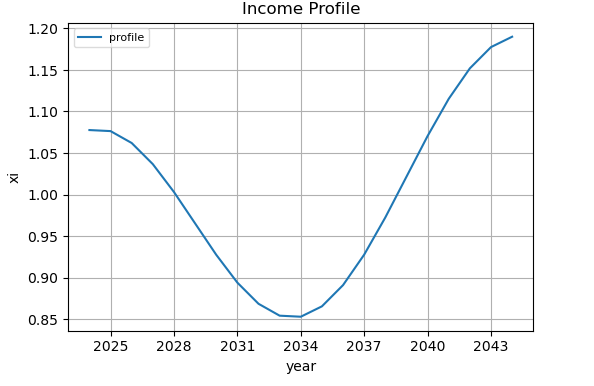
\includegraphics{profile.png}
		\caption{\small Example of a spending profile with 15\% cosine factor and a 12\% linear
		profile. \label{Fig:profile}}
		\end{figure}
\item [$\chi$]
	Factor to reduce spending profile after the passing of one spouse. It is typically
	assumed to be 0.6.
\item [$\rho_{in}$]
	Required minimum distribution for individual $i$ in year $n$. Expressed in fractions
	which are determined from IRS tables. These tables are simple if spouses are less than 10 years apart,
	but a little more complex otherwise, as the age of both spouses need to be taken into account.
	Current implementation only supports spouses being less that 10 years apart.
	An error message is generated in these cases and the calculation is aborted.
\item [$\Gamma_{tn}$]
	Bound for Federal income tax bracket. We define $\Gamma_{(-1)n} := 0$, so that
	$\Gamma_{0n}$ is the upper bound for the 10\% tax bracket in year $n$. As the filing status
		can change for couples, and so can the tax code, $\Gamma_{tn}$ will be changing over $n$.
\item [$\Delta_{tn}$]
	Difference between upper bound $\Gamma_t$ and lower bound $\Gamma_{t-1}$
	of a federal income tax bracket,
	\begin{equation}
		\Delta_{tn} = \Gamma_{tn} - \Gamma_{(t-1)n}.
	\end{equation}
	Once adjusted for inflation,
	the taxable income can be expressed as in Eq.~(\ref{Eq:Tx1}). These data are 7 time series.
	The filing status changes after the passing of one spouse ($n \ge n_d$) and these
	brackets are adjusted accordingly.
\item [$\theta_{tn}$]
	Tax rate for tax bracket $t$ in year $n$. Using $N_t$ time series allows to adjust income
	tax rates in foreseeable future.
	For example, in 2024 the rates (in decimal) are .10, .12, .22, .24, .32, .35, and .37.
	It is speculated that the rates will revert back to 2017 rates in 2026 with
	.10, .15, .25, .28, .33, .35, and .396. See Eq.~(\ref{Eq:IncTax0}) for its use.
\item [$\alpha_{ijkn}$]
	Desired asset allocation for savings account $j$ of individual $i$ in
	assets class $k$ during year $n$.
	Allocation ratios come in many flavors as they could be specified globally between
	individuals and accounts as $\alpha_{kn}$, for example.
	When specified by the user, allocation ratios typically involve two values, one at the
	beginning of the plan $\alpha_{ijk0}$ and the other at the end
	$\alpha_{ijkN_{n-1}}$. Then, intermediate values are interpolated either using
	a linear relation,
\begin{equation}
	\alpha_{ijkn} = a + \frac{n}{N_n - 1} (b - a),
\end{equation}
or an s-curve as in
\begin{equation}
	\alpha_{ijkn} = a + \frac{(b - a)}{2}
	(\tanh((n-n_1)/n_2) + 1),
\end{equation}
	where $n_1$ is the number of years ahead when inflection point will occur, and $n_2$ is the
	width (in years) of the transition. Constants $n_1$ and $n_2$ can be adjusted by the user.
	Default values are $n_1 = 15$, and $n_2 = 5$, meaning that the transition center will occur
	in 15 years, taking place from $15-5$ years to $15+5$ years from now.
	Using $a = \alpha_{ijk0}$ and $b = \alpha_{ijkN_n-1}$ is an approximation as values of $\pm 1$
	are only reached at $\pm \infty$ for a hyperbolic tangent.
	More precise bounds $a'$ and $b'$ for matching the desired start and end values
	can be determined by solving a $2\times 2$ system of equations leading to
	\begin{eqnarray}
		a' &=& (a - k_{12}b')/k_{11} \nonumber \\
		b' &=& ((b - (k_{21}/k_{11})a)/(k_{22} - (k_{21}/k_{11})k_{12}),
	\end{eqnarray}
	where
	\begin{eqnarray}
		k_{11} &=& \frac{1}{2}(1 + \tanh(n_1/n_2)) \nonumber \\
		k_{12} &=& \frac{1}{2}(1 - \tanh(n_1/n_2)) \nonumber \\
		k_{21} &=& \frac{1}{2}(1 - \tanh((N_n-1-n_1)/n_2)) \nonumber \\
		k_{22} &=& \frac{1}{2}(1 + \tanh((N_n-1-n_1)/n_2)).
	\end{eqnarray}
	These interpolation functions allow the allocation ratios to gradually change
	or {\em glide} during retirement. Fig.~(\ref{Fig:allocations}) provides an example
	of an {\em s-curve} gliding allocation ratios.

	\begin{figure}[t]
	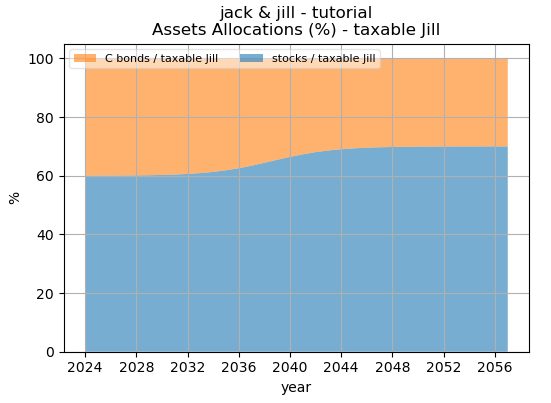
\includegraphics{allocations.png}
		\caption{\small Example of an allocation portfolio with 60/40\% stocks/bonds 
		transitioning to 70/30\% using an s-curve. \label{Fig:allocations}}
	\end{figure}
	It is also possible to have a coarser granularity on the portfolio by
	having an asset allocation scheme
	defined on a sum of accounts. For example, allocation can be coordinated between accounts
	leading to $\alpha_{ikn}$, or even between spouses as $\alpha_{kn}$.
	For any of these cases, it is assumed that weights are always properly scaled so that
	\begin{eqnarray}
		\sum_{k} \alpha_{ijkn} &=& 1, \nonumber\\
		\text{or} \qquad \sum_{k} \alpha_{ikn} &=& 1, \nonumber\\
		\text{or} \qquad \sum_{k} \alpha_{kn} &=& 1,
	\end{eqnarray}
	depending on the scheme selected.

\item [$\Lambda^\pm_{in}$]
	Big-ticket item requested by individual $i$ in year $n$.
	These are large expenses or influx of money
	that can be planned. Therefore, $\Lambda^\pm$ can be positive
	(e.g., sell a house, inheritance) or negative (e.g., buy a house, large gifts).
\item [$\pi_{in}$]
	Sum of pension benefits for individual $i$ in year $n$. These amounts are typically
	specified along with the ages at which these benefits begin. Owl currently assumes
	that pensions are not indexed for inflation, but that functionality can easily be added.
\item [$\zeta_{in}$]
	Social security benefits for individual $i$ in year $n$. Starting age and the passing
	of one individual for spouses will determine the time series. $\bar{\zeta}_{in}$ is
	the same series adjusted for inflation.
\item [$\epsilon_{N_n}$]
	Desired amount to leave as a bequest at the end of the final year of the plan, $N_n-1$,
	which is the beginning of year $N_n$. This amount is the after-tax value of the estate
	for the heirs expressed in today's dollars. See parameter $\nu$ for the heirs tax rate.
\item [$\kappa_{ijn}$]
	Sum of contributions to savings account $j$ made by individual $i$ during year $n$.
	We assume that contributions are made at half-year to balance regular contributions.
	In practice, a contribution
	amount $\kappa_{ijn}$ is specified in which case the contribution to each asset
	class is
	\begin{equation}
		\kappa_{ijkn} = \alpha_{ijkn}\kappa_{ijn}.
	\end{equation}
\item [$\omega_{in}$]
	Sum of wages obtained by individual $i$ during year $n$.
	Do not confuse wages $\omega$ with withdrawals $w$.
\item [$\mu$]
	Dividend return rate in taxable accounts. Average is little above 2\% for S\&P 500.
\item [$\nu$]
	Heirs income tax rate to be applied on the tax-deferred portion of the estate. This is not an estate tax
	but rather the federal income marginal tax rate for the heirs.
\item [$\phi_j$]
	Fraction of savings account $j$ that is left to surviving spouse $i_s$ as a beneficiary
	at the death of individual $i_d$, the first spouse to pass.
\item [$\psi$]
	Income tax rate on long-term capital gain and qualified dividends, typically 15\%.
\item [$\eta$]
	Spousal ratio for surplus deposits, which goes from 0 to 1, as the fraction
	that goes to the $i = 1$ second spouse's account. Therefore, a surplus $s_n$ in year $n$
	will result in a deposit $d$ in the taxable account of individual $i$ as
	\begin{eqnarray}
		\label{Eq:eta}
		d_{0n} & = & (1 - \eta) s_n \nonumber\\
		d_{1n} & = & \eta s_n.
	\end{eqnarray}
	This choice is such that we can set a value depending on the surviving
	individual $\eta = i_s$ for $n \ge n_d$, after the passing of $i_d$.
	Default value is $(N_i - 1)/2$, i.e., $0.5$ for couples and $0$ for single individuals.
	When the beneficiary of the savings accounts is not the other spouse, i.e., 
	when $\phi_j \neq 1, \forall j$, it is recommended that $\eta$ be set to $i_d$ so that
	all surplus get deposited to $i_d$'s accounts,
	thus avoid loopholes when optimizing for the final bequest.
\item [$\mathcal{M}_n$]
	Costs of Medicare and its Income Related Monthly Adjusted Adjustment (IRMAA).
	As this additional adjustment
	is a step function, it would have to be computed using binary variables and mixed-integer linear
	programming. In the current tax code, this adjustment
	depends on the modified adjusted gross income (MAGI) from 2 years earlier. For the
	MAGI, we simply use $G_{n-2} + \bar{\sigma}_{n-2}$ (i.e., gross taxable income
	plus standard deduction from 2 years ago) and ignore the additional IRS
	rules around tax-free interests which are insignificant in most cases.

	There are $q=5$ levels
	of step adjustments adjusted for inflation,
	$\bar{L}_{qn} = L_q\gamma_n$ and each of them introduce
	an annual additional Medicare
	cost of $\bar{C}_{qn} = C_q\gamma_n$, also adjusted for inflation.
	One could use binary variables $z_{inq}$ and the following {\em big M} constraint
	\begin{equation}
		\bar{\sigma}_{n-2} -\bar{L}_{qn} \le z_{inq} M - G_{n-2}
		 \le M - \bar{L}_{qn} + \bar{\sigma}_{n-2},
	\end{equation}
	so that the IRMAA adjustments can be computed as
	\begin{equation}
		\label{Eq:IRMAA}
		\mathcal{M}_n = \sum_{iq} z_{iqn} \bar{C}_{qn}.
	\end{equation}
	If the plan does not have data from 2 years ago as Medicare starts,
	it will use last year's or this year's MAGI instead, in that order.

	While this approach has been implemented and tested, the robustness of the {\em big M} approach
	is not guaranteed. Moreover, the introduction of a large number ($5\times N_i\times N_m$,
        where $N_m$ is the number of years eligible for Medicare) of integer variables with
        disjonctive constraints makes the
	convergence to a solution very slow in most situations.

        A more practical approach is to implement a self-consistent loop that
	optimizes the spending or bequest, and updates the Medicare/IRMAA premiums accordingly.
	Therefore, the value will be computed from the MAGI
	as $\mathcal{M}_n^\ell(G_{n-2} + \bar{\sigma}_{n-2})$, where the value is at iteration $\ell$.
	After only a few iterations, the solution is converging to within a dollar over the
	sum of all variables in the plan. This approach, however, does not guarantee convergence
	as there can be cases where the premiums affect the solution which can oscillate between
	two solutions, but these cases are detected and a slight change in parameters
	solves this issue. As these premiums are introduced as parameters in the constraints,
	there is no direct optimization being performed on Medicare costs.
\end{description}

\section{Intermediate variables}
We use intermediate variables for conciseness or clarity,
but they are ultimately replaced in the final formulation.
All intermediate variables are in uppercase letters.
\begin{description}[leftmargin=4em,style=multiline]
\item [$G_n$]
	Taxable ordinary income in year $n$. Sum of wages, pension, social security benefits, all withdrawals
	from tax-deferred accounts, including Roth conversions, and gains from securities
	(i.e., all gains except those from the $(k=0)$ equities)
	in the ($j=0$) taxable account, including contributions $\kappa$, minus the standard deduction,
	\begin{eqnarray}
		\label{Eq:Tx2}
		G_n &=& 
		\sum_{i} [\omega_{in} + .85\bar\zeta_{in} + \pi_{in}]
		- \bar{\sigma}_n +
		\nonumber \\
		&& \sum_{i} [w_{i1n} + x_{in}] +
		\nonumber \\
		&& \sum_{ik} 
		[(1-\delta(k, 0))(b_{i0n} - w_{i0n} + d_{in} + .5\kappa_{i0n})\alpha_{i0kn}\tau_{kn}]
	\end{eqnarray}
	Social security is indexed for inflation and is assumed to be taxed at 85\%.
	We use a discrete Kronecker $\delta$ function for selecting gains from non-equity assets in
	taxable accounts. These gains are all taxed as ordinary income. Here, we assumed that
	withdrawals and deposits in the taxable account are taking place at the beginning of the year, while
	contributions, if any, are taking place in mid-year.

\item [$Q_n$]
	Qualified dividends and long-term capital gains obtained in year $n$.
	They only involve gains occurring in taxable savings accounts $(j=0)$ that
	were obtained from equities $(k=0)$, or sales of stocks due to withdrawals
	from taxable savings accounts.
	For simplicity, we assume that all equity sales only generate long-term capital gains and
	that all dividends are qualified, resulting in
	\begin{equation}
		\label{Eq:Qx2}
		Q_n = \sum_{i} \alpha_{i00n}\left[(b_{i0n} - w_{i0n} + d_{in} + .5\kappa_{i0n})\mu +
		w_{i0n}{\max(0, \tau_{0n-1})}\right].
	\end{equation}
	A formulation where only a fraction of dividends are qualified can easily be
	implemented with the addition of another parameter.
	Notice that we are using return rates from the previous year.
	The first terms on the right-hand side represent the amount of equities $(k=0)$ in the $(j=0)$
	taxable savings account plus
	half the yearly contributions. The last terms account for withdrawals $w$ of equities assumed
	to have been purchased a year ago. 
	It does not account for losses, but a market drop
	would most likely result in stock purchase rather than sale.
	For withdrawals, we make the assumption of
	selling the most recent stocks which would not be accurate in situations where
	the taxable savings account is being depleted slowly. An implementation keeping track
	of stock purchases and sales is beyond the goal of providing a guide for retirement decisions.

\item [$T_n$]
	Amount of income tax paid on taxable ordinary income $G_n$ in year $n$.
	This is the taxes paid on ordinary income expressed as the sum of the amounts
	paid in each tax bracket as
	\begin{equation}
		\label{Eq:IncTax0}
		T_n = \sum_t f_{tn}\bar{\Delta}_{tn}\theta_{tn}.
	\end{equation}
	Notice that $G_n$ is also defined by Eq.~(\ref{Eq:Tx1}), and that optimal
	values of $f_{tn}$ have to
	minimize $T_n$ when either the bequest or the desired net spending are maximized.
	As the product $\bar{\Delta}_{tn}\theta_{tn}$ does not guarantee to
	be ordered monotonically, a more practical choice is to use the combined variable
	$\bar{F}_{tn} = f_{tn}\bar{\Delta}_{tn}$ in the optimization. Given that the rates on
	tax brackets $\theta_{tn}$ are always increasing monotonically, we are then naturally
	filling in the lower brackets first when optimizing. In that case
	\begin{equation}
		\label{Eq:IncTax1}
		T_n = \sum_t \bar{F}_t \theta_{tn}.
	\end{equation}
\item [$U_n$]
	Amount of income tax paid on long-term capital gains and qualified dividends in year $n$,
	\begin{equation}
		U_n = \psi Q_n.
	\end{equation}
	Although it is not always the case, we assume that qualified dividends and long-term
	capital gains are taxed at the same preferential rate $\psi$.

\end{description}

\chapter{Formulation with imposed asset allocation ratios}
We first present the case where the sums of assets in each savings accounts $b_{ijn}$ are known
over which we assume a prescribed asset allocation ratios.
The amount in each asset class $k$ for $b_{ijkn}$ is simply obtained
from $\alpha_{ijkn} b_{ijn}$ in this case.
This formulation assumes that the accounts are always balanced. This is
a reasonable assumption given the auto-balancing feature offered by many financial service
providers.

The benefit of this approach is that it has less variables and that only the sums of
all asset classes in each savings account need to be known. The rate of return
of the account is then simply the product of the account balance with the sum of
the rates of return weighted according to the desired allocation ratio.
This approach allows us to eliminate $k$ by summing over it and rewrite
\begin{eqnarray}
	\sum_k b_{ijkn+1} &=& \sum_k b_{ijkn} (1 + \tau_{kn}) + \ldots ,
\end{eqnarray}
for the annual evolution of account balances from year $n$ to year $n+1$
as the simpler expression 
\begin{eqnarray}
	b_{ijn+1} &=& b_{ijn} \sum_k \alpha_{ijkn} (1 + \tau_{kn}) + \ldots ,\nonumber \\
		  &=& b_{ijn} (1 + \mathcal{T}_{ijn}) + \ldots ,
\end{eqnarray}
where
\begin{eqnarray}
	\label{Eq:Tau1}
	\mathcal{T}_{ijn} &:=& \sum_k \alpha_{ijkn} \tau_{kn}.
\end{eqnarray}
This is a consequence that the allocation ratios are normalized to unity, i.e.,
\begin{equation}
	\sum_k \alpha_{ijkn} = 1.
\end{equation}
In this formulation where the $\alpha_{ijkn}$ are prescribed,
we will use $\mathcal{T}_{ijn}$ to
add the market returns to the savings balances.

\section{Constraints}
\paragraph*{Required minimum distributions (RMDs)}
	Withdrawals from the ($j=1$) tax-deferred savings accounts must be larger
	or equal than the required minimum distributions, and therefore,
	\begin{equation}
		\label{Eq:C1}
		w_{i1n} -  \rho_{in}b_{i1n} \geq 0.
	\end{equation}
	As $b_{ijn}$ are the balances at the beginning of year $n$, they are also the balances
	at December 31 of the previous year, which is the amount from which the IRS bases the RMDs.
	Eq.~(\ref{Eq:C1}) has to hold for each year $n$ and each individual $i$, and therefore, there
	are $i\times N_n$ such equations (even when $\rho_{in} = 0$).
	These constraints avoid paying the 50\% penalty
	on amounts not withdrawn when RMDs are required.
	Note that aggregate rules need to be considered separately as this approach only considers
	the sum of assets in a class with similar tax treatment (e.g., IRA and 401k).

\paragraph*{Income tax brackets}
	Taxable ordinary income is divided in tax brackets as defined in Eq.~(\ref{Eq:Tx1}), i.e.,
	\begin{eqnarray}
		\label{Eq:C2}
		G_n = \sum_t f_{tn}\bar{\Delta}_{tn} ,\nonumber\\
		0 \leq f_{tn} \leq 1.
	\end{eqnarray}
	Given this definition, all bracket fractions $f$ must be positive and smaller than or equal to 1,
	imposing an upper bound on $f$.
	Because $\theta_{t} > \theta_{t'}$ when $t > t'$, we can exploit
	this monotonically increasing series of rates with $t$ to have the minimization
	algorithm naturally fill the lower tax brackets.
	For that purpose, we need to introduce the combined variable
	\begin{equation}
		\bar{F}_{tn} = f_{tn}\bar{\Delta}_{tn},
	\end{equation}
	implying that
	\begin{equation}
		G_n = \sum_t \bar{F}_{tn},
	\end{equation}
	with
	\begin{equation}
		0 \le \bar{F}_{tn} \le \bar{\Delta}_{tn}.
	\end{equation}
	Then, income tax is easily calculated by Eq.~(\ref{Eq:IncTax1}), 
	\begin{equation*}
		T_n = \sum_t \bar{F}_t \theta_{tn}.
	\end{equation*}

\paragraph*{Account balances}
	Contributions are assumed to be made at half-year to better represent periodic contributions
	made throughout the year. As we already mentioned,
	the account balance at the end of a year is the same as the balance
	at the beginning of the following year.
	Changes include contributions $\kappa$, distributions and withdrawals $w$,
	conversions $x$, surplus deposits $d$, and growth $\tau$ on the account through the year.
	For each spouse $i$, we track each savings account $j$ separately, and tax-deferred accounts
	are coupled to the corresponding tax-exempt account through Roth conversions.

	The timing of Roth conversions, withdrawals, and deposits brings
	additional coupling between these variables, and is worth a detailed discussion.
	First, the financial aspects, and then the algorithmic ones.
	For the former, some financial advisors would recommend making Roth
	conversions at the beginning of the year, while making withdrawals
	at the end. Obviously, financial simulators would always yield higher numbers
	when using this scenario, as the moneys needed to pay the regular bills 
	stayed in the bank until the end of the year. More realistically,
	however, it would be more accurate to assume withdrawals at mid-year,
	to better represent evenly distributed withdrawals. So, financially,
	conversions at the beginning of the year, and withdrawals at mid-year
	make good sense. Conversions are also typically best when
	timed with a market downturns in the year, which are obviously not always at the
	beginning of the year.

	Now, let's look at the optimization side of these transactions.
	During years of positive returns,
	a direct withdrawal from the tax-deferred account at mid-year will always
	be unfavorable when compared to a Roth conversion
	at the beginning of the year, followed
	by a tax-exempt withdrawal later in the same year.
	This is because the second
	scenario involves gains which are tax-free over the half-year, while
	the first one does not. Moving account withdrawals at the beginning
	of the year, and the conversions in mid-year can solve this artificial bias.

	To solve these spurious scenarios, it would be desirable to make the following exclusions
	between surplus $s_n$, withdrawals $w_{ijn}$, and conversions $x_{in}$:
	\begin{eqnarray*}
		s_n &\texttt{XOR} & w_{i0n}, \\
		s_n &\texttt{XOR} & w_{i2n}, \\
		x_{in} &\texttt{XOR} & w_{i2n},
	\end{eqnarray*}
	for $j \neq 1$, i.e., for all withdrawals except those from tax-deferred accounts.
	For example, to favor tax-deferred withdrawals in most reasonable situations,
	it is desirable to make Roth conversions and tax-exempt distributions exclusive events
	by introducing binary variables $z_{in} \in \{0, 1\}$ with the following constraints:
	\begin{alignat}{2}
		\label{Eq:Binary}
		0 & \le \; z_{in}M - x_{in} &\le M, \nonumber \\
		0 & \le \; z_{in}M + w_{i2n} &\le M.
	\end{alignat}
	Here, $M$ is a large number such as $10^7$, just slightly
	larger than what $x$ and $w$ can possibly be.

	Another approach could be to perform Roth conversions at mid-year, while withdrawals
	could be made at the beginning of the year, and surplus deposits,
	if needed due to RMDs or receiving large sums of money,
	could be made at the end of the year. Let's formulate this approach
	in more detail and investigate for potential problems.
	Timing controls which terms get multiplied by the rate of return $(1 + \tau_{kn})$
	for a particular asset $k$.
	Therefore, our current choice would yield
	\begin{eqnarray}
		\label{Eq:C3a}
		b_{ij(n+1)} &=& [b_{ijn} - w_{ijn} + .5\kappa_{ijn}](1 + \mathcal{T}_{ijn})
		+ [\delta(j, 2) - \delta(j, 1)]x_{in} (1 + \mathcal{T}_{ijn}/2)
		\nonumber \\
		&& 
		+\ \delta(j, 0) d_{in} + .5 \kappa_{ijn},
	\end{eqnarray}
	where we use discrete Kronecker $\delta$ functions for selecting the specific accounts involved
	in Roth conversions. These conversions are made such that asset allocation
	ratios in the sending and receiving accounts are unchanged.

	Bringing all variables
	to the left-hand side, this gets rewritten as
	\begin{eqnarray}
		\label{Eq:C3}
		b_{ij(n+1)} - (b_{ijn} - w_{ijn}) (1 + \mathcal{T}_{ijn})
		&& \nonumber \\
		-\ [\delta(j, 2) - \delta(j, 1)]x_{in}(1 + \mathcal{T}_{ijn}/2)
		-\ \delta(j, 0) d_{in}
		&=& \kappa_{ijn} (1 + \mathcal{T}_{ijn}/2).
	\end{eqnarray}

	When $j=0$, this equation introduces
	a path to shelter negative returns by performing an over-withdrawal from the taxable
	account at the beginning of the year followed by a deposit in the
	same account at the end of the year. This can 
	be removed by using another binary variable, thus making these events exclusive by using
	the same strategy as Eq.~(\ref{Eq:Binary}).

	A much simpler approach, while not so natural,
	is to move all transactions to be synchronous at the beginning or at the end of the year
	thus avoiding undesirable movements of funds.
	If we select the beginning of the year, this leads to
	\begin{eqnarray}
		\label{Eq:C3b}
		b_{ij(n+1)} - b_{ijn}(1 + \mathcal{T}_{ijn}) 
		&& \nonumber \\
		- \ [\delta(j, 0)d_{in} - w_{ijn} + (\delta(j, 2) - \delta(j, 1))x_{in}] (1 + \mathcal{T}_{ijn})
		&=& \kappa_{ijn} (1 + \mathcal{T}_{ijn}/2).
	\end{eqnarray}
	This is the current approach used in Owl.

	The initial balances $\beta_{ij}$ are one of the main inputs of the model.
	The initial savings account balances are imposed through additional constraints as
	\begin{eqnarray}
		\label{Eq:InitialBalance}
		b_{ij0} = \beta_{ij}.
	\end{eqnarray}
	At this point, we assume that all accounts are balanced according to the desired
	allocation ratios $\alpha_{ijkn}$.

	We also introduce another constraint that might look unnecessary, but helps
	convergence, and prevents overdrafts during the year of passing of the first spouse.
	As withdrawals and conversions are at the beginning of the year 
	we impose that
	\begin{eqnarray}
		w_{ijn} + \delta(j, 1)x_{in} \le b_{ijn}.
	\end{eqnarray}

\paragraph*{Roth Conversions}
	Roth conversions cannot be larger than the balance at the beginning of the year in the account:
	\begin{equation}
		x_{ijn} \le b_{i1n}.
	\end{equation}
	This constraint, however, is naturally satisfied when $b_{ijn} \ge 0$ non-negativity bounds are enforced.
	Additional maximum Roth conversion constraints $x_{max}$ can be imposed by the user and
	then the previous equation becomes
	\begin{equation}
		x_{in} \le \min(b_{i1n}, x_{max}).
	\end{equation}

\paragraph*{Net spending}
	For calculating the net spending $g_n$, we consider the cash flow of all withdrawals,
	wages, social security and pension benefits, and big-ticket items. 
	Then we subtract potential surplus $s_{n}$ and all taxes and Medicare premiums paid:
	\begin{eqnarray}
		g_n = \sum_i [\omega_{in} + \bar{\zeta}_{in} + \pi_{in} ] 
		+ \sum_{ij} w_{ijn} + \sum_i \Lambda^\pm_{in} - s_{n}
		- T_n - U_n - \mathcal{M}^\ell_n.
	\end{eqnarray}
	When both spouses are alive, surplus $s_n$ gets deposited in the taxable accounts
	according to variable $\eta$ as described in Eq.~(\ref{Eq:eta}),
	\begin{equation}
		\label{Eq:eta2}
		d_{in} = [\delta(i, 0)(1 - \eta) + \delta(i, 1)\eta] s_n .
	\end{equation}
	Otherwise, for $n \ge n_d$, variable $\eta$ gets redefined as $\eta = \delta(1, i_s)$.

	Notice how big-ticket items $\Lambda^\pm$ contribute directly to the cash flow.
	Replacing intermediate variables and bringing all variables to the left-hand side, we get
	\begin{eqnarray}
		\label{Eq:C4}
		g_n - \sum_{ij} w_{ijn} + s_{n}
		+ \sum_t \bar{F}_{tn} \theta_{t n} &&\nonumber \\
		+ \psi\alpha_{i00n} \sum_{i} \left[\mu(b_{i0n} - w_{i0n} + d_{in})
		+ w_{i0n}\max(0, \tau_{0n-1})\right] 
		&=& \sum_i [\omega_{in} + \bar{\zeta}_{in} + \pi_{in} ] \nonumber\\
		&& + \sum_i [\Lambda^\pm_{in} - .5\psi\alpha_{i00n}\mu\kappa_{i0n}] \nonumber\\
		&& - \mathcal{M}_n^\ell.
	\end{eqnarray}
	Notice that we do not consider market losses as we use $\max(0, \tau)$, and that
	rates from only the previous year are used. Tax-loss
	harvesting is beyond the scope of this model, as is the tracking of stocks
	purchased over the years.
	For clarity, we did not express $\mathcal{M}_n^\ell(G_n+\bar{\sigma}_n)$ in terms of the modified
	adjusted gross income (MAGI), but this term is there to indicate that there is a self-consistent
	loop solving for it and that we are at iteration $\ell$.

	We want the net spending to be predictable and smooth. We use
\begin{equation}
	\label{Eq:C5a}
	g_{n}/\bar{\xi}_{n} = g_0/\bar{\xi}_0,
\end{equation}
where the net spending is adjusted for inflation and where we use the time series of parameter $\xi_n$ 
allowing for additional adjustments to the overall desired spending.
Note that $\bar{\xi}_0 = \xi_0$ as $\gamma_0=1$.
This spending profile is used to lower the desired income by a reduction factor $\chi$
after the passing of one spouse and/or to allow for more realistic spending profiles, such as
the {\em smile} profile described above.
Eq.~(\ref{Eq:C5a}) can be rewritten as
\begin{equation}
	\label{Eq:C5}
	g_n \xi_0 - g_0 \bar{\xi}_n = 0,
\end{equation}
for the constraints to be enforced. Once $g_0$ is determined, the whole time series of net spending
is determined.

\paragraph*{Taxable ordinary income}
	We connect the two definitions for $G_n$ stated above in Eqs.~(\ref{Eq:Tx1}) and (\ref{Eq:Tx2}),
	\begin{eqnarray}
		\sum_t f_{t n}\bar{\Delta}_{t n} &=&
		\sum_i [\omega_{in} + .85\bar\zeta_{in} + \pi_{in}]  \nonumber \\
		&& + \sum_{i} [w_{i1n} + x_{in} ]
		\nonumber\\
		&& + \sum_{ik} [(1 - \delta(k, 0))(b_{i0n} - w_{i0n} + d_{in} + .5\kappa_{i0n})\alpha_{i0kn}\tau_{kn}] - \bar{\sigma}_n,
	\end{eqnarray}
	and re-arrange to move variables to the LHS as follows
	\begin{eqnarray}
		\label{Eq:C6}
		\sum_t \bar{\Delta}_{t n} f_{t n}
		- \sum_{i} [ w_{i1n} + x_{in}] &&
		\nonumber \\
		- \sum_{ik} [(1 - \delta(k, 0))(b_{i0n} - w_{i0n} + d_{in})\alpha_{i0kn}\tau_{kn}] &=&
		\sum_i [\omega_{in} + .85\bar\zeta_{in} + \pi_{in} ] 
		- \bar{\sigma}_n
		\nonumber \\
		&& + .5\sum_{ik} [(1-\delta(k, 0))\alpha_{i0kn}\tau_{kn}\kappa_{i0n}].
	\end{eqnarray}

\chapter{Mapping of decision variables}
At this point, one can use one of the many algebraic modeling languages
such as AMPL, GAMS, MOSEK, AIMMS, and Gurobi, and code the equations above
using that language, but most of these applications are
proprietary and require a license and additional software installation.
These languages allow the problem to be stated at a high level and
steps to cast the problem in a form suitable for solution are performed automatically.
There are also object-oriented language extensions, such as Python's Pyomo
and PuLP that can ease the process of solving these problems.
For completeness, however, we present here a simple
index mapping approach that allows solving this problem using a generic
linear programming solver.

Using a simple interface for mapping sparse objects to dense ones, the approach described here
has been successfully tested with both the HiGHS open-source solver
and the MOSEK proprietary solver.
To cast the problem in a form suitable for a linear programming solver, we will use
a single block vector represented by the array $y[q()]$ with index-mapping functions $q()$.
While this process can be achieved using slicing and reshaping in some programming
languages, we will present a generic approach suitable for most programming languages.
The detailed approach presented here also allows us to determine the size of the problem to solve.
We proceed alphabetically for all variables, and continue to use the convention of having
index 0 for representing the first element.

To bring all variables in a single block vector,
we will simply use two generic index mapping functions defined as
\begin{equation}
	q_*(C, \ell_1, \ell_2, \ell_3 ; N_1, N_2, N_3) :=
	C + \ell_1N_2N_3 + \ell_2N_3 + \ell_3 ,
\end{equation}
and
\begin{equation}
	q_C(C, N_1, N_2, N_3) :=
	C + N_1N_2N_3,
\end{equation}
with the constraint that $0 \le \ell_i < N_i$.

\paragraph*{Account balances (\boldmath$b$)}
For storing the savings account balances appropriately, variable $b_{ijn}$ needs to have one
more entry $(N_n + 1)$ to
store the end-of-life estate value. Therefore, we use
\begin{equation}
	y[q_b(i, j, n)] = b_{ijn},
\end{equation}
where
\begin{equation}
	\label{Eq:Extra}
	q_b(i, j, n) = q_*(C_b, i, j, n; N_i, N_j, N_n+1)
\end{equation}
and where $n$ exceptionally runs from 0 to $N_n$ inclusively, and therefore
$q_b$ runs from $C_b = 0$ to $C_{d} - 1$,
where
\[
	C_{d} = q_C(C_b, N_i, N_j, N_n+1) = [N_i N_j (N_n+1)].
\]

\paragraph*{Surplus deposits (\boldmath$d$)}
For the surplus deposits in the taxable savings accounts $d_{in}$ we will use
\begin{equation}
	y[q_d(i, n)] = d_{in},
\end{equation}
where
\begin{equation}
	q_d(i, n) = q_*(C_d, i, n, 0; N_i, N_n)
\end{equation}
with $q_d$ running from $C_d$ to $C_f - 1$, where
\[
	C_f = q_C(C_d, N_i, N_n, 1) = [N_i(N_j(N_n+1) + N_n)].
\]

\paragraph*{Tax bracket fractions (\boldmath$f$)}
For tax bracket fractions $f_{t n}$ we will use
\begin{equation}
	y[q_f(t, n)] = f_{t n},
\end{equation}
where
\begin{equation}
	q_f(t, n) = q_*(C_f, t, n, 0; N_t, N_n, 1)
\end{equation}
with $q_f$ running from $C_f$ to $C_g - 1$, where
\[
	C_g = q_C(C_f, N_t, N_n, 1) = [N_i(N_j(N_n+1) + N_n) + N_tN_n].
\]

\paragraph*{Net spending (\boldmath$g$)}
For net spending $g_{n}$ we will use
\begin{equation}
	y[q_g(n)] = g_{n},
\end{equation}
where
\begin{equation}
	q_g(n) = q_*(C_g, n, 0, 0; N_n, 1, 1) = C_g + n,
\end{equation}
with $q_g$ running from $C_g$ to $C_s - 1$, where
\[
	C_s = q_C(C_g, N_n, 1, 1) = [N_i(N_j(N_n+1) + N_n) + (N_t + 1) N_n].
\]

\paragraph*{Surplus (\boldmath$s$)}
Surplus can be generated if big-ticket items are received (inheritance, sale of a house, etc.)
or due to RMDs. Surplus $s$ is then deposited to taxable savings accounts according
to variable $\eta$. We will use
\begin{equation}
	y[q_s(n)] = s_{n},
\end{equation}
where
\begin{equation}
	q_s(n) = q_*(C_s, n, 0, 0; N_n, 1, 1) = C_s + n,
\end{equation}
with $q_s$ running from $C_s$ to $C_w - 1$, where
\[
	C_w = q_C(C_s, N_n, 1, 1) = [N_i(N_j(N_n+1) + N_n) + (N_t + 2) N_n].
\]

\paragraph*{Withdrawals (\boldmath$w$)}
For withdrawals $w_{ijn}$ we will use
\begin{equation}
	y[q_w(i, j, k, n)] = w_{i j n},
\end{equation}
where
\begin{equation}
	q_w(i, j, n) = q_*(C_w, i, j, n; N_i, N_j, N_n)
\end{equation}
with $q_w$ running from $C_w$ to $C_x - 1$, where
\[
	C_x = q_C(C_w, N_i, N_j, N_n) = [N_i(N_j(2N_n + 1) + (N_t + 2) N_n].
\]

\paragraph*{Roth conversions (\boldmath$x$)}
Finally, for Roth conversions $x_{in}$ we will use
\begin{equation}
	y[q_x(i, n)] = x_{i n},
\end{equation}
where
\begin{equation}
	q_x(i, n) = q_*(C_x, i, n, 0; N_i, N_n, 1)
\end{equation}
with $q_x$ running from $C_x$ to $C_* - 1$, where
\[
	C_* = q_C(C_x, Ni, N_n, 1) = [N_i(N_j(2N_n + 1) + (N_t + N_i + 2) N_n].
\]

Adding $N_z=2$ binary variables $z_{inz}$ adds $N_zN_iN_n$ more decision variables.
With $N_i = 2, N_j = 3, N_k = 4, N_t = 7$ we have $27 N_n + 6$ variables. For
a 30-year plan, this results in 816 decision variables. If the time resolution is increased to
months, that would result in 9,726 variables which is still solvable by today's standards.

\section{Reverse mapping of indices}
The inverse functions for the index-mapping functions will be derived for the
most complex case encountered in this paper.
If we have
\begin{equation}
	z = q_*(C, i, j, k, n; N_i, N_j, N_k, N_n) := C + iN_jN_kN_n + jN_kN_n + kN_n + n,
\end{equation}
then $(i, j, k, n) = q_*^{-1}(z; N_i, N_j, N_k, N_n, C)$ is obtained from
\begin{eqnarray}
	n &=& \texttt{mod}(\texttt{mod}(\texttt{mod}(z - C, N_jN_kN_n), N_kN_n), N_n), \nonumber \\
	k &=& \texttt{mod}(\texttt{mod}(z - C - n, N_jN_kN_n), N_kN_n)/N_n, \nonumber \\
	j &=& \texttt{mod}(z - C - n - kN_n, N_jN_kN_n)/(N_kN_n), \nonumber \\
	i &=& (z - C - n - kN_n - jN_kN_n)/(N_jN_kN_n).
\end{eqnarray}
While this holds for all cases presented in the previous section, this can be easily simplified
for cases having fewer active indices. However, some modern languages can accomplish this
mapping rather easily by providing \texttt{reshape()} functions.

\chapter{Building constraint matrices}
Let's first define generic index-mapping functions $I$ and $J$ as
\begin{eqnarray}
	\label{Eq:Offsets}
	I_l(n) &=& C_l + n, \nonumber \\
	I_l(i, n; N_n) &=& C_l + iN_n + n, \nonumber \\
	I_l(i, j, n; N_j, N_n) &=& C_l + iN_j N_n + jN_n +n, \\
	\ldots &=& \ldots \nonumber
\end{eqnarray}
and so on, which would cumulatively increase row count $C_l$ at each new instance $l$,
similar to how we proceeded in the previous section.
This allows us to build rectangular matrices by iteratively adding rows.
These constraint matrices have $C_*$
columns but will have less rows,
forming an underdetermined system to be optimized using linear programming.

\section{Inequality constraints}

\paragraph*{Required minimum distributions (RMDs)}
We rewrite the inequality constraint on required minimum distributions
Eq.~(\ref{Eq:C1}) using matrix $A_{u}y \le u$ starting with the following $N_iN_n$ rows, 
\begin{eqnarray}
	A_u[I_0(i, n), q_w(i, 1, n)] &=& -1 \nonumber \\
	A_u[I_0(i, n), q_b(i, 1, n)] &=& \rho_{in}, \nonumber \\
	u[I_0(i, n)] &=& 0, \\
	&&\qquad\forall i \in \{0,\ldots, N_i-1\}, \nonumber\\
	&&\qquad\forall n \in \{0,\ldots, N_n -1\},\nonumber
\end{eqnarray}
and all other elements in the same rows of $A_u$ being $0$.
Notice that while $b$ has $N_n+1$ elements, the constraints
for $b$ go from $0$ to $N_n-1$ as there is no RMD required in the last year of the plan $N_n$.
See Eq.~(\ref{Eq:Extra}).

\paragraph*{Income tax brackets}
Similarly, we add $N_t N_n$ more rows to matrix $A_uy \le u$ to express
the inequality constraint in Eq.~(\ref{Eq:C2})
setting an upper limit on fractions $f_{t n} \le 1$.
Instead of using $f$, however, we will use $F_{tn} = f_{tn}\bar{\Delta}_{tn}$
of the same dimensions and therefore,
\begin{eqnarray}
	A_u[I_1(t, n), q_F(t, n)] &=& 1, \nonumber \\
	u[I_1(t, n)] &=& \bar{\Delta}_{tn},\\
	&&\qquad\forall t \in \{0,\ldots, N_t-1\}, \nonumber\\
	&&\qquad\forall n \in \{0,\ldots, N_n -1\},\nonumber
\end{eqnarray}
and all other elements in the same rows of $A_u$ being $0$.

\section{Equality constraints}

\paragraph*{Account balances}
For the equality constraint on account balances expressed in Eq.~(\ref{Eq:C3}),
we will define an equality constraint matrix $A_ey = v$ starting
with $N_iN_jN_n$ rows as
\begin{eqnarray}
	\label{Eq:B1}
	A_e[J_0(i, j, n), q_b(i, j, n+1)] &=& 1, \nonumber \\
	A_e[J_0(i, j, n), q_b(i, j, n)] &=& -(1 + \mathcal{T}_{ijn}), \nonumber \\
	A_e[J_0(i, j, n), q_x(i, n)] &=& -(\delta(j, 2) - \delta(j, 1))(1 + \mathcal{T}_{ijn}), \nonumber \\
	A_e[J_0(i, j, n), q_w(i, j, n)] &=& (1 + \mathcal{T}_{ijn}), \nonumber \\
	A_e[J_0(i, j, n), q_d(i, n)] &=& -\delta(j, 0)(1 + \mathcal{T}_{ijn}), \\
	&&\qquad\forall i \in \{0,\ldots, N_i-1\},\nonumber\\
	&&\qquad\forall j \in \{0,\ldots, N_j-1\},\nonumber\\
	&&\qquad\forall n \in \{0,\ldots, N_n-1\}, \nonumber
\end{eqnarray}
where $v$ is
\begin{equation}
	v[J_0(i, j, n)] = \kappa_{ijn}(1 + \mathcal{T}_{ijn}/2).
\end{equation}
The initial account balances expressed in Eq.~\ref{Eq:InitialBalance} are imposed through
\begin{eqnarray}
	A_e[J_1(i, j, k), q_b(i, j, 0)] &=& 1, \nonumber \\
	v[J_1(i, j, k)] &=& \beta_{ijk},  \\
	&&\qquad\forall i \in \{0,\ldots, N_i-1\},\nonumber\\
	&&\qquad\forall j \in \{0,\ldots, N_j-1\},\nonumber\\
\end{eqnarray}
leading to $N_i N_j$ additional rows to $A_e$.

\paragraph*{Net spending}
For the equality constraint on net spending expressed in Eq.~(\ref{Eq:C4}),
we add $N_n$ more rows to $A_ey = v$ as
\begin{eqnarray}
	A_e[J_2(n), q_g(n)] &=& 1, \nonumber \\
	A_e[J_2(n), q_w(i, j ,n)] &=& -1 + \delta(j, 0)\psi\alpha_{i00n}(\max(0, \tau_{0n-1}) - \mu), \nonumber \\
	A_e[J_2(n), q_d(i, n)] &=& 1 + \psi\mu\alpha_{i00n}, \nonumber \\
	A_e[J_2(n), q_F(t, n)] &=& \theta_{t n}, \nonumber \\
	A_e[J_2(n), q_b(i, 0, n)] &=& \psi\mu\alpha_{i00n}, \nonumber \\
	&&\qquad\forall t \in \{0,\ldots, N_t-1\},\nonumber\\
	&&\qquad\forall i \in \{0,\ldots, N_i-1\},\nonumber\\
	&&\qquad\forall j \in \{0,\ldots, N_j-1\},\nonumber\\
	&&\qquad\forall n \in \{0,\ldots, N_n-1\}, \nonumber
\end{eqnarray}
where $v$ is
\begin{equation}
	v[J_2(n)] = \sum_i [\omega_{in} + \bar\zeta_{in} + \pi_{in}
	+ \Lambda^\pm_{in} - .5\psi\mu\alpha_{i00n}\kappa_{i0n}] - \mathcal{M}_n^\ell.
\end{equation}

The condition of having a predictable net spending expressed as an
equality in Eq.~(\ref{Eq:C5}) adds $N_n-1$ more rows to $A_ey = v$ as
\begin{eqnarray}
	A_e[J_3(n), q_g(0)] &=& -\bar{\xi}_n, \nonumber \\
	A_e[J_3(n), q_g(n)] &=& \xi_0, \nonumber \\
	v[J_3(n)] &=& 0, \\
	&&\qquad\forall n \in \{1,\ldots, N_n\}. \nonumber
\end{eqnarray}

\paragraph*{Taxable ordinary income}
Finally, for the equality constraint in Eq.~(\ref{Eq:C6}) establishing taxable
ordinary income, we add $N_n$ rows to $A_ey = v$ as follows
\begin{eqnarray}
	A_e[J_4(n), q_F(t, n)] &=& 1, \nonumber \\
	A_e[J_4(n), q_w(i, 1, n)] &=& -1, \nonumber \\
	A_e[J_4(n), q_b(i, 0, n)] &=&  (1 - \delta(k, 0))\alpha_{i0kn}\tau_{kn}, \\
	A_e[J_4(n), q_w(i, 0, n)] &=& -(1 - \delta(k, 0))\alpha_{i0kn}\tau_{kn}, \nonumber \\
	A_e[J_4(n), q_d(i, n)] &=&     (1 - \delta(k, 0))\alpha_{i0kn}\tau_{kn}, \nonumber \\
	A_e[J_4(n), q_x(i, n)] &=& -1, \nonumber \\
	&&\qquad\forall t \in \{0,\ldots, N_t-1\},\nonumber\\
	&&\qquad\forall i \in \{0,\ldots, N_i-1\},\nonumber\\
	&&\qquad\forall k \in \{0,\ldots, N_k-1\},\nonumber\\
	&&\qquad\forall n \in \{0,\ldots, N_n-1\}, \nonumber
\end{eqnarray}
with
\begin{eqnarray}
	v[J_4(n)] &=& 
	\sum_i [\omega_{in} + .85\bar\zeta_{in}  + \pi_{in}]
	+ .5\sum_{ik} [(1-\delta(k, 0))\alpha_{i0kn}\tau_{kn}\kappa_{i0n}]
	- \bar{\sigma}_n.
\end{eqnarray}

\section{Other considerations}
\paragraph*{Beneficiaries}
Tax-exempt and tax-deferred accounts have special tax rules that allow giving part
or the entire value of
tax-exempt accounts to a spouse who can then consider it as his/her own.
These accounts typically use percentages to designate beneficiaries.
Let $\phi_j$ be the fraction of the account $j$ that a spouse $i_d$ wishes
to leave to his/her surviving spouse $i_s$
in the year $n_d  - 1 < N_n - 1$ following the year of passing. 
To account for that event in year $n_d$, Eq.~(\ref{Eq:C3b}) needs to be rewritten as
\begin{eqnarray}
	b_{ij(n+1)} &=& (1 - \delta(n, n_d-1)\delta(i, i_d)) \nonumber \\
	&&\times \Bigl\{\left[b_{ijn} - w_{ijn} + \delta(j, 0)d_{ij}\right](1 + \mathcal{T}_{ijn})
	+ \left[(\delta(j, 2) - \delta(j, 1))x_{in} + \kappa_{ijn}\right](1 + \mathcal{T}_{ijn}/2) 
	\Bigr\}\nonumber \\
	&& + (\phi_j\delta(n, n_d-1)\delta(i, i_s)) \nonumber  \\
	&& \times \Bigl\{\left[b_{i_djn} - w_{i_djn} + \delta(j, 0)d_{i_dn}\right](1 + \mathcal{T}_{i_djn})
	\nonumber\\
	&& + \left[(\delta(j, 2) - \delta(j, 1))x_{i_dn} + \kappa_{i_djkn}\right](1 + \mathcal{T}_{i_djn}/2) 
	\Bigr\}.
\end{eqnarray}
The first multiplier $()$ on the right-hand side will always be one except for $i_d$ in
year $n_d-1$ when it will be zero. This will result in emptying all accounts for $i_d$ for years
$n_d$ and beyond.
The second special multiplier $()$ before the second set of curly braces
$\{\}$ will always be zero except for the surviving
spouse $i_s$ in year $n_d-1$, who will then inherit a fraction $\phi_j$ of account $j$ that
was scheduled to go into $i_d$'s $j$ account at the beginning of year $n_d$.

Rewriting the last equation as a constraint results in
\begin{eqnarray}
	&&b_{ij(n+1)} 
	  \nonumber  \\
	&& - (1 - \delta(n, n_d-1)\delta(i, i_d)) \nonumber\\
	&& \times \Bigl\{ \left[b_{ijn} - w_{ijn} + \delta(j, 0)d_{in} \right](1 + \mathcal{T}_{ijn})
	+ \left[(\delta(j, 2) - \delta(j, 1))x_{ikn}\right](1 + \mathcal{T}_{ijn}/2) \Bigr\}
	\nonumber \\
	&&- (\phi_j\delta(n, n_d-1)\delta(i, i_s)) \nonumber \\
	&& \times \Bigl\{ \left[b_{i_djn} w_{ijn} + \delta(j, 0)d_{in}\right](1 + \mathcal{T}_{i_djn})
	+ \left[(\delta(j, 2) - \delta(j, 1))x_{i_dkn}\right](1 + \mathcal{T}_{i_djn}/2) \Bigr\}
	\nonumber \\
	&=& \left[(1 - \delta(n, n_d-1)\delta(i, i_d)) \kappa_{ijn} (1 + \mathcal{T}_{i_djn}/2) \right.
	\nonumber\\
	&& + \left.(\phi_j\delta(n, n_d-1)\delta(i, i_s))
	\kappa_{i_djn}\right](1 + \mathcal{T}_{i_djn}/2).
\end{eqnarray}
We are now ready to replace Eq.~(\ref{Eq:B1}) for $A_ey = v$ by
\begin{eqnarray}
        \label{Eq:B2}
        A_e[J_0(i, j, n), q_b(i, j, n+1)] &=& 1, \nonumber \\
        A_e[J_0(i, j, n), q_b(i, j, n)] &=& - (1 - \delta(n, n_d-1)\delta(i, i_d))
		(1 + \mathcal{T}{ijn}), \nonumber \\
        A_e[J_0(i, j, n), q_w(i, j, n)] &=& (1 - \delta(n, n_d-1)\delta(i, i_d))
	(1 + \mathcal{T}_{ijn}),\nonumber \\
        A_e[J_0(i, j, n), q_d(i, j, n)] &=& - (1 - \delta(n, n_d-1)\delta(i, i_d))
		\delta(j, 0) (1 + \mathcal{T}_{ijn}), \nonumber \\
        A_e[J_0(i, j, n), q_x(i, n)] &=& - (1 - \delta(n, n_d-1)\delta(i, i_d))
                (\delta(j, 2) - \delta(j, 1)),
		(1 + \mathcal{T}_{ijn}/2), \nonumber \\
		\text{when $N_i =2$ and $i = i_s$,} && \nonumber\\
        A_e[J_0(i, j, n), q_b(i_d, j, n)] &=& - (\phi_j\delta(n, n_d-1)\delta(i, i_s))
		(1 + \mathcal{T}_{i_djn}), \nonumber \\
        A_e[J_0(i, j, n), q_w(i_d, j, n)] &=& (\phi_j\delta(n, n_d-1)\delta(i, i_s))
	(1 + \mathcal{T}_{i_djn}), \nonumber\\
        A_e[J_0(i, j, n), q_d(i_d, n)] &=&  -(\phi_j\delta(n, n_d-1)\delta(i, i_s))
		\delta(j, 0)(1 + \mathcal{T}_{i_djn}), \nonumber \\
        A_e[J_0(i, j, n), q_x(i_d, n)] &=& - (\phi_j\delta(n, n_d-1)\delta(i, i_s))
                (\delta(j, 2) - \delta(j, 1))
		(1 + \mathcal{T}_{i_djn}/2), \nonumber \\
                \nonumber \\
        &&\qquad\forall i \in \{0,\ldots, N_i-1\},\nonumber\\
        &&\qquad\forall j \in \{0,\ldots, N_j-1\},\nonumber\\
        &&\qquad\forall n \in \{0,\ldots, N_n-1\}, \nonumber
\end{eqnarray}
where $v$ is
\begin{eqnarray}
	v[J_0(i, j, n)] 
	&=& (1 - \delta(n, n_d-1)\delta(i, i_d)) \kappa_{ijn}(1 + \mathcal{T}_{ijn}/2)
	\nonumber \\
	&& + (\phi_j\delta(n, n_d-1)\delta(i, i_s))\kappa_{i_djn}(1 + \mathcal{T}_{i_djn}/2). 
\end{eqnarray}
While the last two equations may look cumbersome, their net effect is only to include
a few more terms when $n=n_d-1$. 

\paragraph*{Assets allocation ratios}
When asset allocation ratios $\alpha$ are imposed,
they should also be applied to how
contributions amounts $\kappa_{ijn}$ are invested, such that 
\begin{equation}
	\kappa_{ijkn} = \alpha_{ijkn} \kappa_{ijn}.
\end{equation}
For other allocation schemes, just substitute $\alpha_{ijkn} = \alpha_{ikn}$ or $\alpha_{kn}$
depending on the scheme selected.

Assets allocation have been handled easily by assuming that
the accounts are always rebalanced
and only using a single multiplier $\mathcal{T}$, defined as
\begin{equation}
	\mathcal{T}_{ijn} = \sum_k \alpha_{ijkn}\tau_{kn},
\end{equation}
to compute to return
on the total balance of each savings account.

\paragraph*{Spousal deposits and withdrawals}
In order to keep the problem linear, a simple constraint that can be imposed on
surplus deposits to be made in taxable savings accounts is to specify a spousal ratio $\eta$
such as
\begin{equation}
	d_{0n} = \eta d_{1n}.
\end{equation}
A similar spousal ratio can be imposed on withdrawals from tax-deferred accounts
\begin{equation}
	w_{01n} = \eta w_{11n},
\end{equation}
but this can cause drawing from an account empty while the other spousal account is not.

\chapter{Objective functions}
The objective function is a simple scalar defined as $c\cdot y$ that will be minimized.

\paragraph*{Maximum net spending}
There are a few ways by which a retirement plan can be optimized. For maximizing the net spending under
the constraint of a desired bequest, we introduce the following relation
\begin{equation}
	\label{Eq:Bequest}
	E_n = \sum_{ij} (1 - \nu\delta(j, 1)) b_{ijn},
\end{equation}
which is the value of the estate in nominal dollars at year $n$,
taking into consideration the heir's marginal income tax rate on the ($j=1$) tax-deferred account. 
In this situation, the concept of surplus deposit remains valid to handle
surplus income.

For a desired bequest $\epsilon_{N_n}$, expressed in today's
dollars, the final amount in year $N_n$ will need to be
\begin{equation}
	E_{N_n} = \bar\epsilon_{N_n} = \epsilon_{N_n} \gamma_{N_n}.
\end{equation}
Fixing a bequest value amounts to adding the following constraint
\begin{equation}
	\sum_{ij} b_{ijN_n} (1 - \nu\delta(j, 1)) = \epsilon_{N_n} \gamma_{N_n},
\end{equation}
which would add one more row to $A_ey = v$ as
\begin{eqnarray}
	A_e[I(0), q_b(i, j, N_n)] &=& (1 - \nu\delta(j, 1)) \nonumber \\
	v[I(0)] &=& \epsilon_{N_n}\gamma_{N_n} \\
	&&\qquad\forall i \in \{0,\ldots, N_i-1\},\nonumber\\
	&&\qquad\forall j \in \{0,\ldots, N_j-1\},\nonumber\\
\end{eqnarray}
where $I(0)$ is used only to provide the proper row offset $C_l$. See Eq.~(\ref{Eq:Offsets}).

For maximizing the net spending under the constraint of a fixed bequest, one has simply to
minimize the inner product $c\cdot y$, where $c$ is
\begin{eqnarray}
	c[q_g(0)] &=& -1,
\end{eqnarray}
and 0 otherwise. See Eq.~\ref{Eq:C5}.

\paragraph*{Maximum bequest}
If, on the other hand, one would like to maximize the bequest under the constraint of a desired net spending $g_o$,
one would add the following row to $A_ey = v$
\begin{eqnarray}
	\label{Eq:FixedIncome}
	A_e[I(0), q_g(0)] &=& 1, \nonumber \\
	v[I(0)] &=& g_o.
\end{eqnarray}

The objective function would then be derived from Eq.~(\ref{Eq:Bequest}) as
minimizing the inner product $c\cdot y$, where $c$ is
\begin{eqnarray}
	\label{Eq:MaxBequest}
	c[q_b(i, j, N_n)] &=& -(1 - \nu\delta(j, 1)),\\
	&&\qquad\forall i \in \{0,\ldots, N_i-1\},\nonumber\\
	&&\qquad\forall j \in \{0,\ldots, N_j-1\},\nonumber\\
\end{eqnarray}
and 0 otherwise.

\end{document}
